\section{Successes}
\subsection{BERT}
\begin{frame}[c]{BERT: Bidirectional Encoder Representations}
    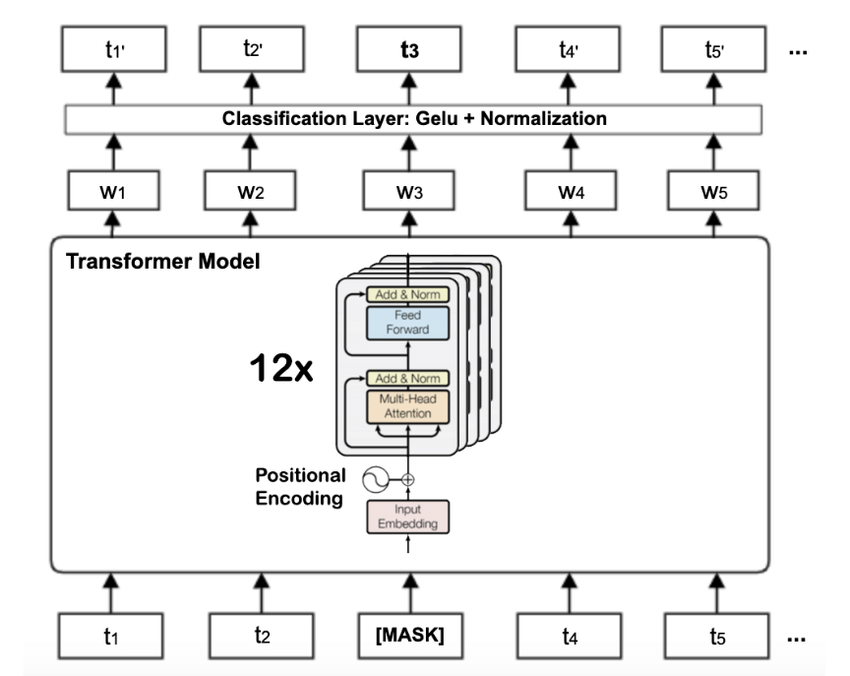
\includegraphics[height=0.8\textheight]{bert} \\
    \gray{Image Source: \cite{khalid_rubert_2021}}
    \large
    Original BERT \cite{devlin_bert_2018}
    \pnote{
        BERT is an encoder-only transformer
    }
\end{frame}

\subsection{GPT}
\begin{frame}[c]{GPT: Pure Decoder Architectures}
    \begin{columns}
        \column{0.4\textwidth}
        \begin{minipage}[c][\textheight][c]{\linewidth}
            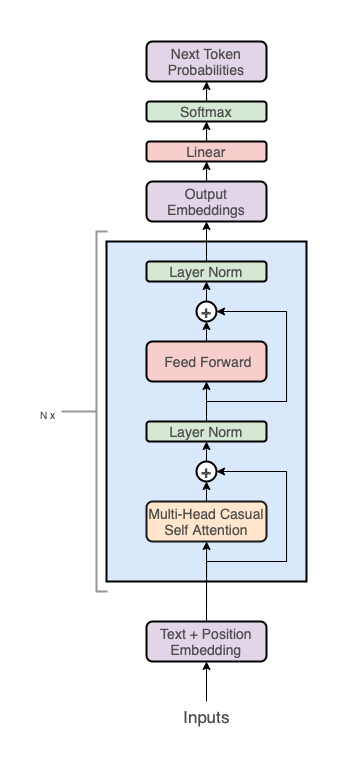
\includegraphics[height=0.8\textheight]{GPT_architecture} \\
            \gray{Image Source: \cite{mody_gpt_2023}}
        \end{minipage}
        \column{0.6\textwidth}
        \begin{minipage}[c][\textheight][c]{\linewidth}
            \large
            Examples:
            \begin{itemize}
                \item GPT \cite{radford_improving_2018}
                \item GPT2 \cite{radford_language_2019}
                \item GPT3? \cite{brown_language_2020}
                \item GPT4? \cite{openai_gpt4_2023}
                \item LlaMa \cite{touvron_llama_2023}
                \item Bloom \cite{workshop_bloom_2022}
                \item OPT \cite{zhang_opt_2022}
                \item PaLM \cite{chowdhery_palm_2022}
            \end{itemize}
        \end{minipage}
    \end{columns}
    \pnote{
        GPT3 is a question mark, but we pretty much know most about it \\
        GPT4 is a bigger question, but I have a slide for that too
    }
\end{frame}


\begin{frame}[c]{GPT4: What We Know}
    \begin{itemize}[<+(1)->]
        \item Parameters: 1.76 trillion, about 10x of GPT3
        \item Mixture of Experts (MoE) with 16 partially differently trained
            heads with 111B parameters each, asking only two for each forward
            pass
        \item Trained on 13 trillion tokens, maybe more
        \item Speculation of training costs of the final run are 63 million USD.
        \item Performance got a lot worse through lobotomization from RLHF (ChatGPT4) and using proposal networks to reduce inference costs
    \end{itemize}
    \pause
    No official source ... most of it is based on speculation from what george hotz leaked in an interview \cite{transhumanismvideos_george_2023}
    \pnote{
        Only the first two bullet points where directly from george hotz
    }
\end{frame}

\subsection{CLIP}
\begin{frame}[c]{CLIP: Multimodal Embedding Spaces}
    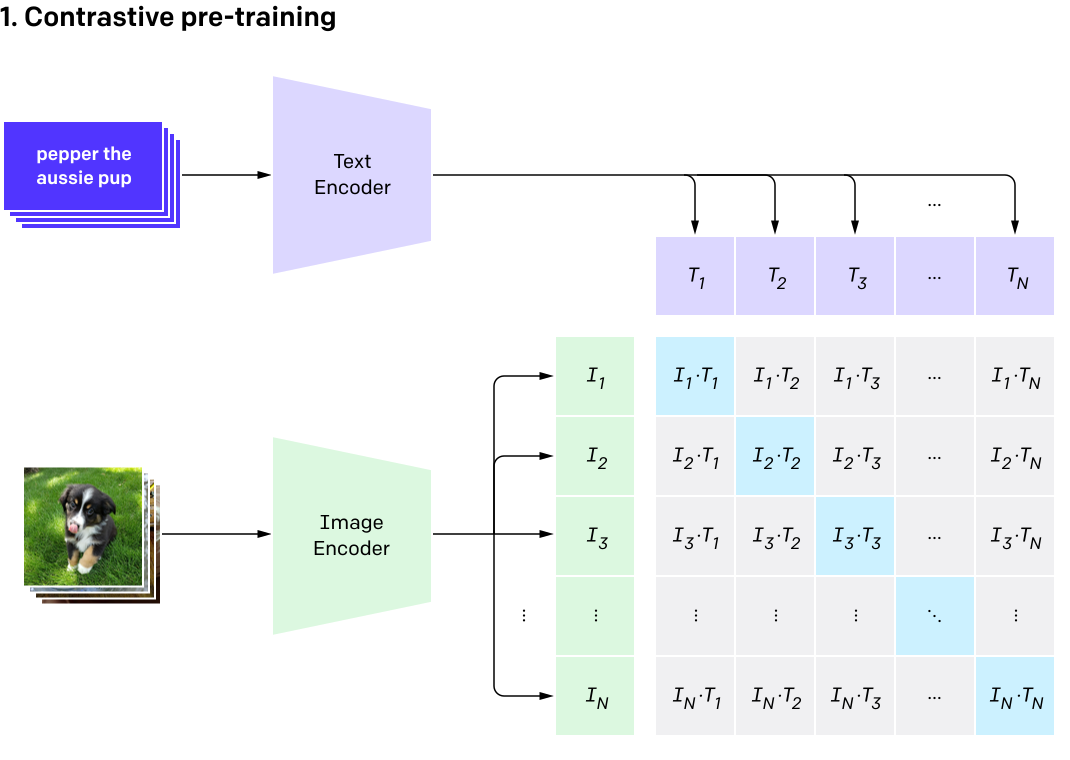
\includegraphics[height=0.8\textheight]{clip} \\
    \gray{Image Source: \cite{radford_learning_2021}}
    \large We can now describe images!
    \pnote{
        we now have an shared embedding between text and images \\
        \\
        Specifically we can determine \\
        how well a description matches an image
    }
\end{frame}

\subsection{Latent Diffusion Models}
\begin{frame}[c]{Latent Diffusion Models}
    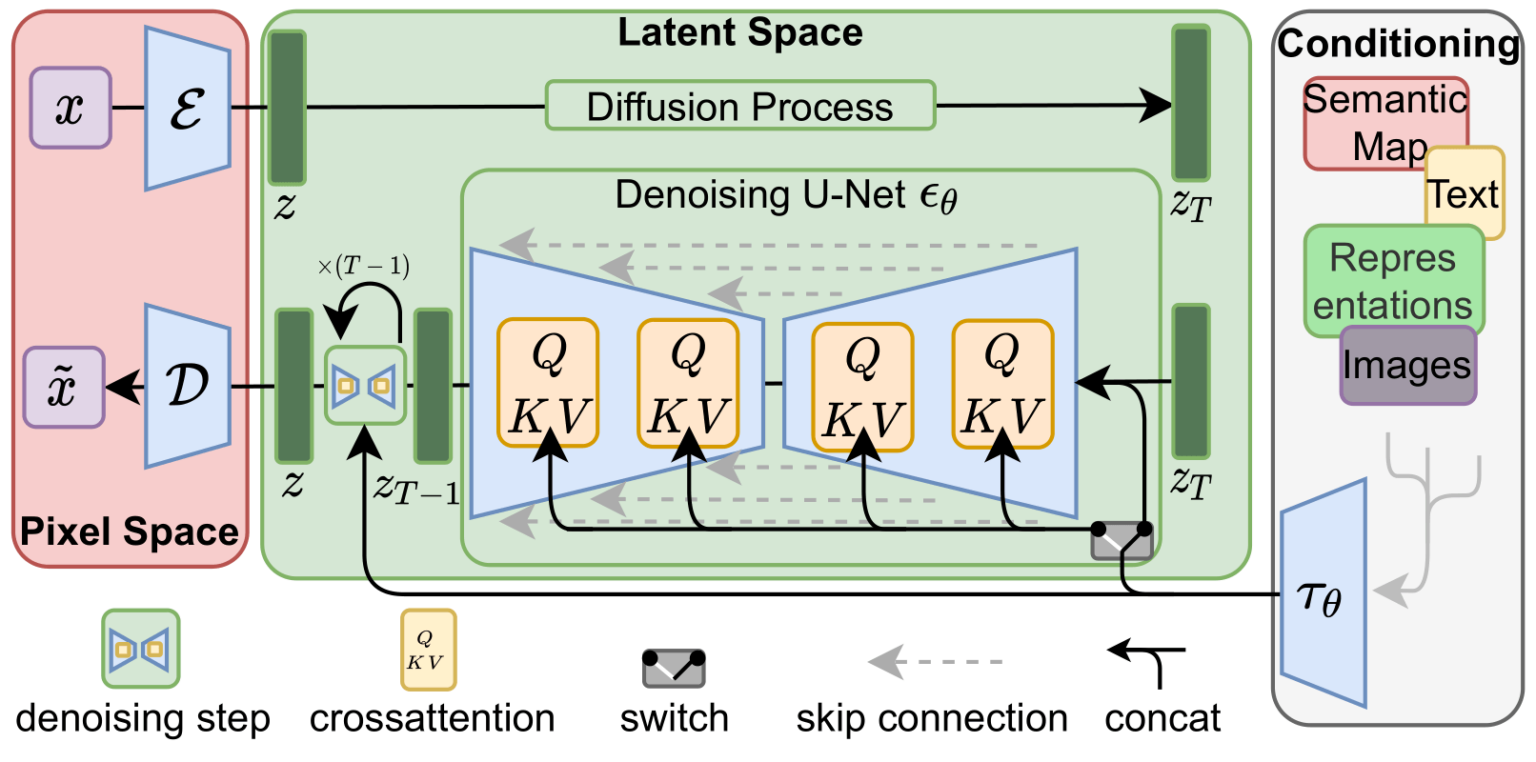
\includegraphics[width=\textwidth]{stable_diffusion} \\
    \gray{Image Source: \cite{rombach_highresolution_2022}}
    \large We can now generate images! \\
    \normalsize
    (We can also do that using GANs \cite{esser_taming_2021})
    % Generating images based on shared semantic embeddings
    % Diffusion \cite{sohl-dickstein_deep_2015}
\end{frame}

\subsection{Reinforcement Learning}
\begin{frame}[c]{GATO: A Generalist Agent}
    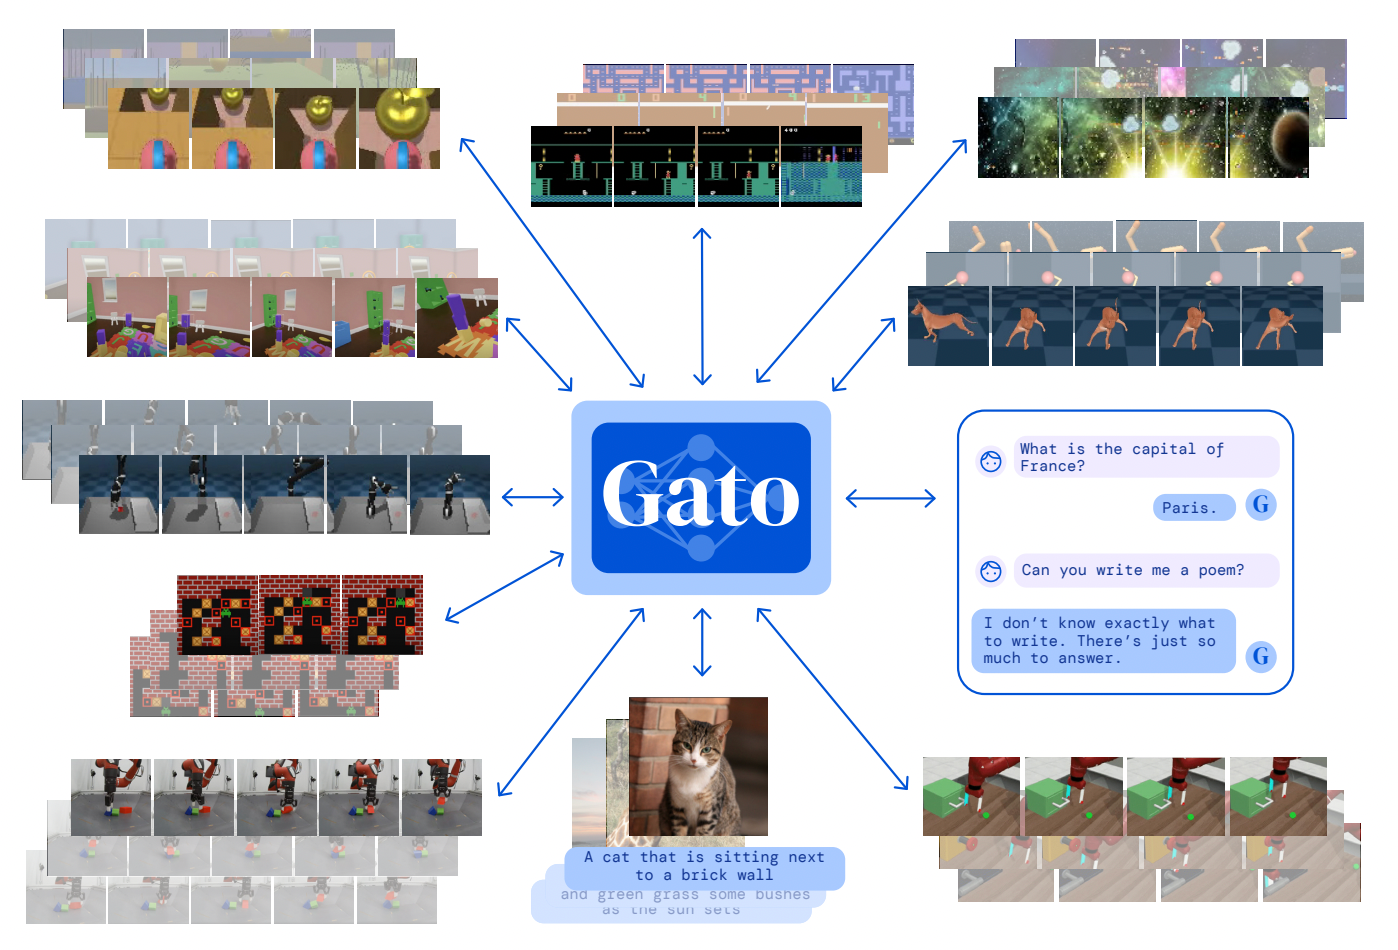
\includegraphics[height=0.8\textheight]{gato} \\
    \gray{Image Source: \cite{reed_generalist_2022}}
    \pnote{
        And more recently something something model-based RL
    }
\end{frame}

\subsection{Physics Simulation}
\begin{frame}[c]{Physics Simulation in Latent Spaces}
    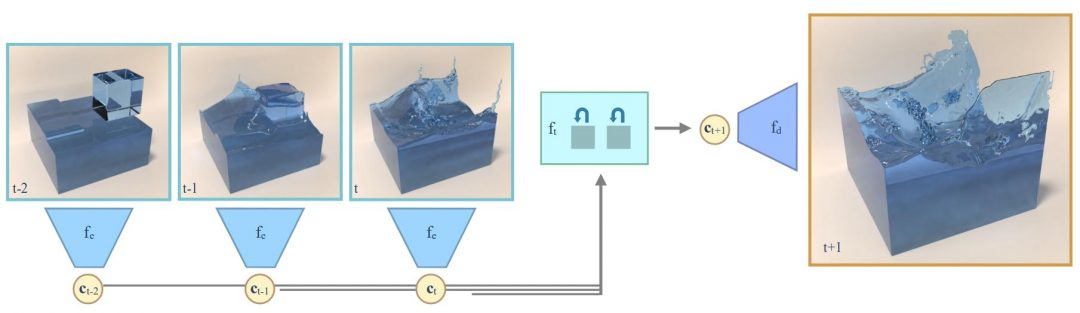
\includegraphics[height=0.8\textheight,width=\textwidth,keepaspectratio]{lsp} \\
    \gray{Image Source: \cite{wiewel_latent_2019}}
    \large
    \begin{aquote}{Latent Space Physics \cite{wiewel_latent_2019}}
        ... we arrive at a data-driven solver that yields practical speed-ups, and
        at its core is more than 150x faster than a regular pressure solver.
    \end{aquote}
    \pnote{
        Speed up simulation by 150x 
    }
\end{frame}

\subsection{Capability}

\begin{frame}[c]{Current Progress is Exponential}
    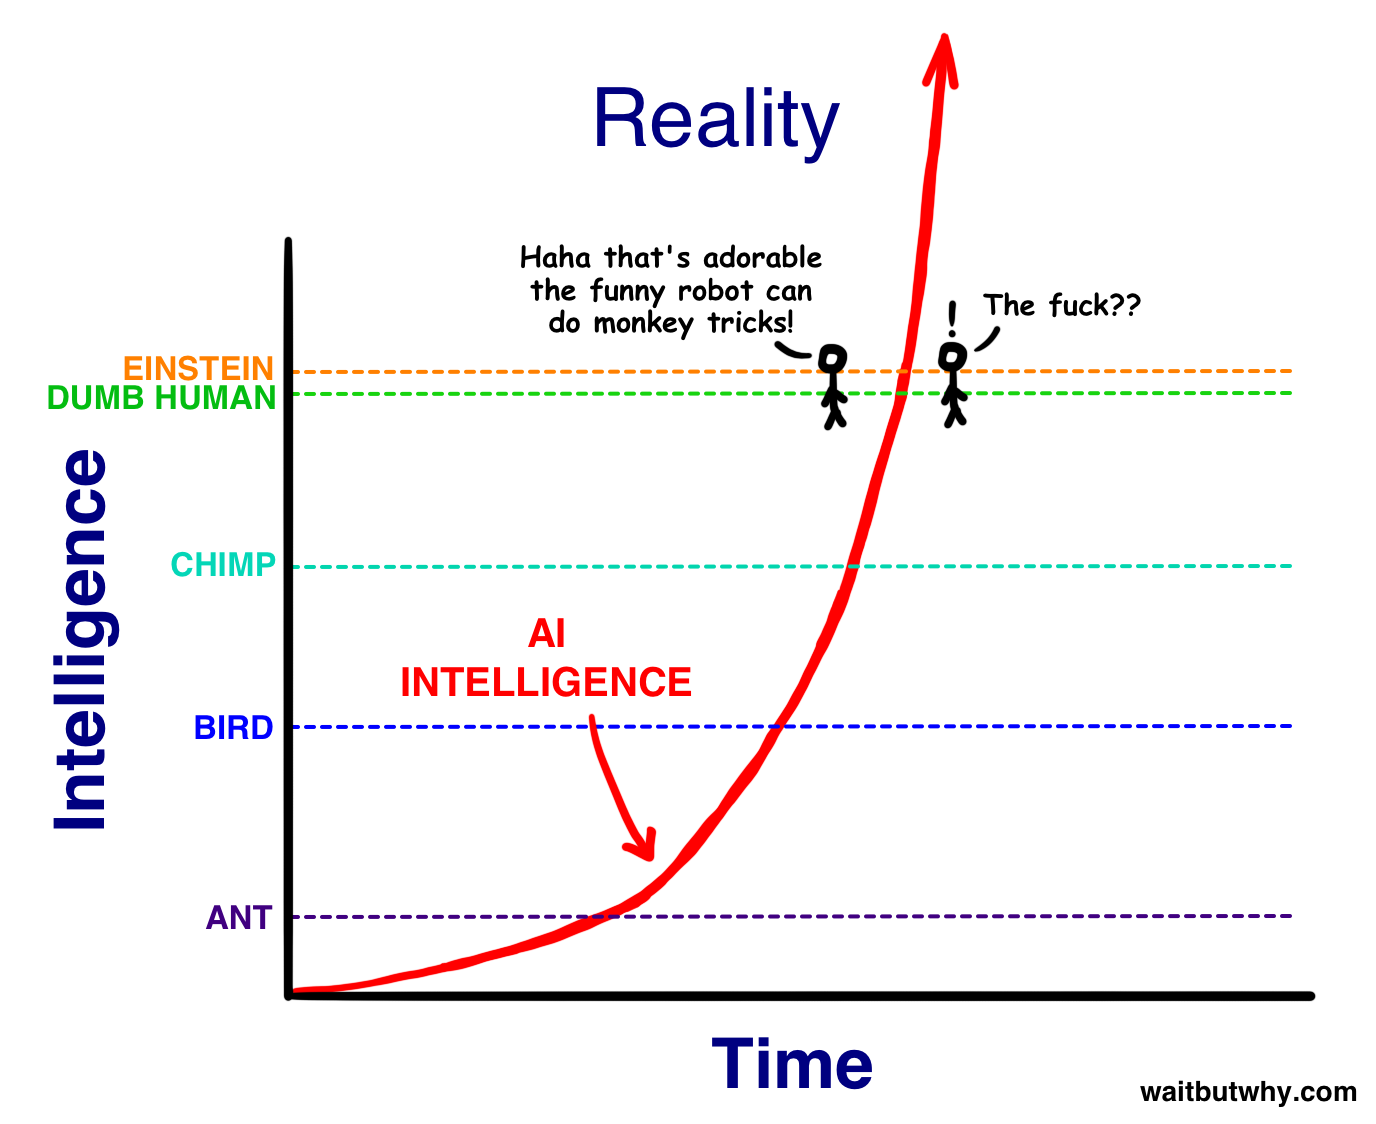
\includegraphics[height=0.8\textheight]{Intelligence2} \\
    \gray{Image Source: \cite{urban_artificial_2015}}
\end{frame}

% \subsection{Meta Cognition}
% \begin{frame}[c]{Reflexion}
%     Reflexion \cite{shinn_reflexion_2023}
%     \todo{include architecture}
% \end{frame}

% \begin{frame}[c]{Architecture Changes}
%     \begin{itemize}[<+(1)->]
%         \item No Encoder part, GPTs are autoregressive decoder-only
%         \item LayerNorm before, not after Layers
%         \item Positional Encoding for each intermittent Layer 
%     \end{itemize}
% \end{frame}
